Sicherheitsrisiken in virtualisierten Netzinfrastrukturen lassen sich auf verschiedene Weisen wie z.B. nach ISO/OSI-Schicht, nach Verletzung der klassischen C.I.A.-Aspekte, nach Schicht in der NV-Architektur, oder aus Sicht des SPs bzw. InPs klassifizieren. Da dieses Kapitel sich aber auf durch Netzvirtualisierung gegenüber herkömmlichen Netzinfrastrukturen neu hinzukommende Risiken konzentriert, liegt der folgenden Klassifizierung zur Verdeutlichung der Angriffsrichtungen die in Abbildung \ref{fig:gefahren_klassifizierung} dargestellte Struktur zugrunde, die sich auf der Drei-Schichtenarchitektur der Netzwerkvirtualisierung (Abbildung \ref{fig:gefahren_dreiEbenenDerVirtualisierung}) ableitet.

Sicherheitsrisiken werden zunächst nach solchen technischer, organisatorischer bzw. unternehmerischer und rechtlicher Art geordnet. Im Zentrum der Betrachtung stehen dabei die technischen Risiken, welche wiederum nach Angriffsrichtungen ‚\textit{von NI ausgehend}‘, ‚\textit{von VN/VM ausgehend}‘ und ‚\textit{vom User ausgehend}‘ gegliedert werden. In jeder dieser Kategorien wird nach Angriffsziel ‚\textit{gegen NI}‘, ‚\textit{gegen VN/VM}‘ und ‚\textit{gegen User}‘ unterteilt. \\
Da die Kategorien ‚\textit{I.1 von NI ausgehend gegen NI}‘ und ‚\textit{III.3 vom User ausgehend gegen User}‘ in virtualisierten Netzwerkumgebungen keine neuen Angriffsszenarien eröffnen, werden sie hier dem Ziel des Kapitels entsprechend nicht tiefergehend ausgeführt. 


\begin{figure}[htb]
	\begin{center}
	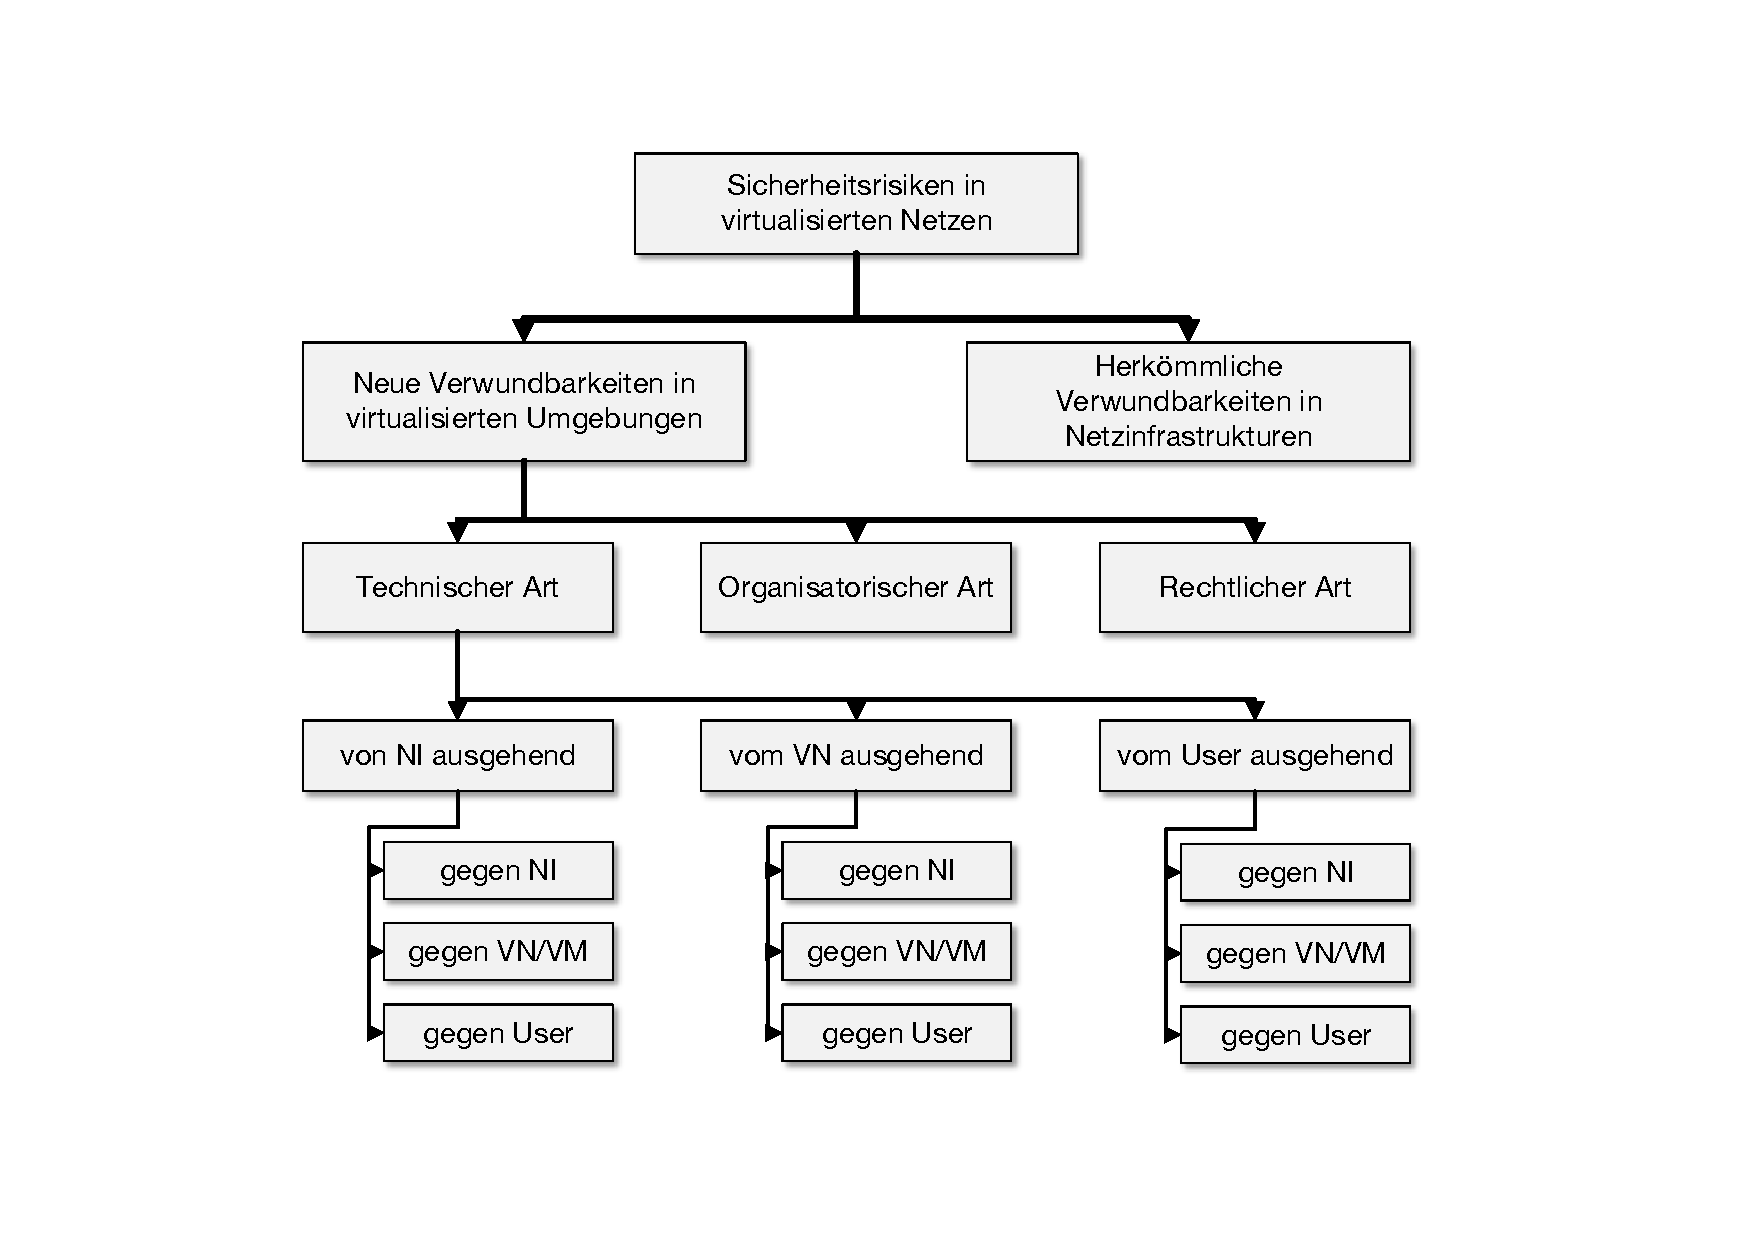
\includegraphics[width=\textwidth]{gefahren_klassifizierung.pdf}
	\caption{\label{fig:gefahren_klassifizierung} Klassifizierung von Gefahren in virtualisierten Netzwerken
		\newline NI = Netzwerkinfrastruktur / Substratnetz. Der physische Host einer VM ist Teil der NI.
		\newline User = Endsystem bzw. in VNs implementierter Service oder Nutzer
		\newline Kategorie I.1 und III.3 beinhalten keine durch NV neu hinzukommenden Risiken.}
	\end{center}
\end{figure}





\subsubsection{Technischer Art}
\label{subsubsec:gefahren_virt_technisch}
Dieses Kapitel analysiert sich durch NV ergebende Sicherheitsrisiken, die auf Netzwerk- oder Virtualisierungstechnologie basieren.
Der Kapitelaufbau folgt der Klassifizierung in Abbildung \ref{fig:gefahren_klassifizierung}. 


\paragraph{I.2 \& I.3 Von NI ausgehend gegen VN/VM und User.}
\label{parag:vonNI}
Physische Hosts bieten ihren VMs Ressourcen an. Alle Dienste und Anwendungen der VMs werden letztlich auf dem physischen Host ausgeführt und auch alle Daten auf ihm gespeichert. Dies eröffnet ihm prinzipiell die Möglichkeit eines Monitorings der VM-Aktivitäten, was ab einer gewissen Intensität über Verwaltungsbelange hinausgehen und Privats"-phären"-anforderungen widersprechen wird. Auf demselben Weg lassen sich auch vertraulichkeitsverletzende Sniffing- oder Spoofing-Attacken gegen VM bzw. VN starten. \\
Da alle ihre Rechenoperationen letztlich auf dem physischen Host ausgeführt werden, ist es für eine VM nur schwer möglich, sich gegen solche Angriffe zu wehren. Eine Verschlüsselung der eigenen Daten kann einer VM nicht ohne Weiteres helfen, da auch die Schlüsseldatei innerhalb der VM und damit auf dem physischen Host gespeichert werden muss.\\
Auch Manipulation des legitimen Datenverkehrs, (gezieltes) Verwerfen von empfangenen Paketen bzw. das Einschleusen schadhafter Nachrichten bieten dem Host eine weitere Möglichkeit der Kompromittierung, gegen die VNs und Endsysteme wohl schutzlos ausgeliefert sind.
%\underline{[AUSFÜHRLICHER?]}\\
Durch derartige Aktionen oder auch unzureichende Sicherungsmaßnahmen gegen Datenabfluss kann der physische Host in den SLAs vereinbarte Bestimmungen verletzen, was gerade bei Drittanbietern als Hostingpartner eine Rolle spielt.




\paragraph{Von VN/VM ausgehend}
\label{parag:vonVN}
Die gemeinsame Nutzung von Ressourcen wie Speicher und Netzwerkkarten eröffnet VMs neue Angriffsmöglichkeiten gegen ihr Substratnetz, gegen andere VNs/VMs und gegen User.


\begin{itemize}
\item \textbf{II.1 Von VN/VM ausgehend gegen NI/ihren physischen Host.~~}
Das Bereitstellen von Ressourcen für VMs ist auch für den physischen Host nicht ohne Risiko. Schadhafte oder bösartige VMs können Verwundbarkeiten ihres physischen Host über zugeteilte Ressourcen angreifen. Ohne hinreichende Restriktionen kann eine VM über ihr zugeteiltes Kontingent hinaus bspw. wichtige Speicherbereiche manipulieren oder z.B. durch übermäßige Reservierung von CPU-Zeiten eine Denail of Service Attacke gegen den physischen Host bzw. das Substratnetz fahren. Da Host und virtuelle Netztopologie aus der Ferne konfigurierbar sind, stellt das Einschleusen von konstruierten Nachrichten des verwendeten Netzwerkmanagementprotokolls auf oder durch die Netzwerkkarte des physischen Hosts einen weiteren gefährlichen Angriffsvektor dar.\\
Nach Eindringen in oder Übernahme des Hosts -- einem „break of isolation“ im ersten Sinne \cite{wu2010network} -- könnte eine schadhafte VM dann ihr Kontingent an Ressourcen beeinflussen, netztopologische Informationen sammeln, andere Netzwerkressourcen oder -infrastrukturkomponenten angreifen und so beispielsweise Dienste anderer VMs oder VNs behindern.

\item \textbf{II.2 Von VN/VM ausgehend gegen VN/VM.~~}
Neben den herkömmlichen Angriffsszenarien zwischen Maschinen im selben Netzwerk, ergeben sich v. a. aus der gemeinsamen Nutzung von Ressourcen neue Angriffsvarianten.\footnote{Da die Angriffstechniken von VMs gegen VMs auf anderen physischen Hosts vergleichbar mit herkömmlichen Angriffen in nicht-virtualisierten Netzinfrastrukturen sein dürften, werden hier hauptsächlich VMs auf demselben physischen Host betrachtet.} 
Ein Angreifer kann sich nun gezielt Ressourcen auf denjenigen physischen Maschinen mieten, auf denen auch sein Angriffsziel gehostet wird, um so erleichterten Zugang zu dessen Verwundbarkeiten zu erlangen. Durch Eindringen oder Übernehmen gewisser Ressourcen des gemeinsamen physischen Hosts kann eine schadhafte VM ggfs. Verwundbarkeiten anderer VMs ausnutzen oder durch Cross-VN-side-channel-Attacken vertrauliche Informationen gewinnen und Daten manipulieren. Ein Beispiel einer Integritätsverletzung mittels einer solchen Attacke findet sich in \cite{ristenpart2009hey}. \\
Da i.d.R. nur virtuelle Netzwerkkarten zugeteilt werden, kann jede VM potentiell den gesamten Datenverkehr aller VMs bzw. VNs auf derselben physischen Netzwerkkarte lesen. Ein Monitoring anderer VMs auch aus anderen VNs, ein „break of Isolation“ im zweiten Sinne bedroht deren Vertraulichkeit. Durch Belauschen des Netzwerkverkehrs lassen sich ggfs. auch Dienste gemeinsam gehosteter VN reproduzieren und dadurch bspw. ein live Videostreaming breiter zugänglich machen. \cite{natarajansecurity}\\
Sollte es einer VM gelingen kritische Teile ihres physischen Hosts zu übernehmen, so stehen ihr zusätzlich die im Abschnitt \textit{\nameref{parag:vonNI}} aufgeführten Angriffsvektoren offen.


\item \textbf{II.3 Von VN/VM ausgehend gegen User.~~}
Auch ein virtuelles Netzwerk kann mit herkömmlichen Methoden wie Monitoring der Nutzeraktivitäten oder dem Einschleusen von konstruierten Nachrichten zur Störung oder Abbruch von Peer-to-Peer-Verbindungen Einfluss auf den Nutzverkehr seiner User nehmen.
\end{itemize}



\paragraph{Vom User ausgehend}
\label{parag:vonUser}
Einem Benutzer oder schadhaften Anwendungsprogramm stehen auch in virtualisierten Netzwerkumgebungen die bekannten Methoden der Störung durch z.B. Herbeiführen von Überlastsituationen in VN oder NI offen.

\begin{itemize}
	\item \textbf{III.1 Vom User ausgehend gegen NI.~~}
	Da sich die virtuelle Netztopologie im VNE-Prozess laufend ändert, müssen Netzwerkkomponenten wie Switches und Router dynamisch umprogrammierbar sein. Dies jedoch ermächtigt Angreifer solche ggfs. mit Codeexpliots wie Bufferoverflows o. Ä. zu kompromittieren und für ihre Zwecke zu nutzen oder einen Denail of Service herbeizuführen.\\
	Daneben besteht die Chance auch Netzwerkknoten anzugreifen. Gelingt es z.B. mit einem Rootkit wie BluePill \cite{rutkowska2008bluepilling} -- als Vorbereitung für weitere Angriffe -- einen Hypervisor zu übernehmen, wird so gleichzeitig die Kontrolle über alle gehosteten VMs erlangt. Auch eine VM lässt sich als Rootkit instrumentalisieren. \cite{wu2010network}
	\item \textbf{III.2 Vom User ausgehend gegen VN/VM.~~}
	Aus der dynamischen Natur virtueller Netzwerktopologien ergeben sich neue Verwundbarkeiten: Während der Migration im Livebetrieb eines VNs ist eine Man-in-the-Middle-Attacke möglich, mit der Informationen über und Inhalte des migrierenden VNs erlangt werden können. \cite{natarajansecurity} Auch die Manipulation von Speicherbereichen der VMs ist während der Migration umsetzbar und lässt sich sogar automatisieren. \cite{oberheide2008empirical}\\
	Die Notwendigkeit die gesamte virtuelle Netzwerkstruktur aus der Ferne umkonfigurieren zu können, erschließt weitere Angriffsziele: Attacken auf die VN-Ma"-nagement"-tools durch z.B. Cross-Site-Scripting, SQL-Injection etc. werden lohnend, da auf diese Weise effizient Kontrolle über das gesamte Netzwerk gewonnen werden kann.	
\end{itemize}


Neben solchen technischen Sicherheitsrisiken eröffnen sich durch NV aber auch solche organisatorischer und rechtlicher Art.


\subsubsection{Organisatorischer Art}
\label{subsubsec:gefahren_virt_organisatorisch}
Unter ‚organisatorischen‘ Risiken werden hier Risiken für Unternehmen verstanden, die im Zusammenhang mit Virtualisierung stehen.

Wie im Kapitel \ref{subsubsec:gefahren_virt_technisch} dargestellt, eröffnet Netzvirtualisierung eine Reihe neuer Verwundbarkeiten für gehostete Systeme. Gerade für Unternehmen stellt die teils deutliche Gefähr"-dung der Vertraulichkeit und Integrität von Firmen- oder Kundendaten ein ernstzunehmendes Problem dar. Da Netzvirtualisierung oftmals via Cloudcomputing abgewickelt wird, erhöht sich das Risiko eines Datenlecks nochmals durch den Up- und Downloadprozess von Daten.\\
Mögliche Richtlinien zur Beschränkung von Anzahl, Art oder Eigentümer gemeinsam gehosteter VNs/VMs, welche sich z.B. als komplexe Sicherheitsvektoren mit dem Algorithmus aus Kapitel \ref{subsec:ansatz2} oder als ,,medium''-Knotenlevel mit dem in \ref{subsec:ansatz1} vorgestellten realisieren ließen, schränken Flexibilität der Netzarchitektur und Kostenvorteil der NV zwar ein, können jedoch bei ausreichendem Sicherheitslevel der physischen Hosts einen gewissen Schutz gewährleisten. Vor- und Nachteile eines solchen Ansatzes werden in Kapitel \ref{subsec:ansatz2} und \ref{subsec:svne_vergleich} diskutiert.

Ein großer Vorteil virtueller Maschinen besteht in der Leichtigkeit Momentaufnahmen (Snapshots) für Backup- oder Migrationszwecke zu erstellen. Beim Wiedereinspielen dieser werden jedoch ggfs. zwischenzeitlich deaktivierte Accounts, veraltete Sicherheitsrichtlinien oder mittlerweile gepatchte Schwachstellen wieder produktiv gesetzt. Organisationen müssen hierfür einen geeigneten Prozess etablieren, der auch das Patchmanagement häufig offline gehender VMs regelt. Der Umgang mit solchen VMs ist schwierig, da Würmer z.B. relativ schnell alle verwundbaren Systeme infizieren. Geht die VM danach offline wird Malware darin ggfs. nicht entdeckt und die Wurminfektionselle startet erneut beim Onlinegehen der VM. \cite{garfinkel2005virtual} 



\subsubsection{Rechtlicher Art}
\label{subsubsec:gefahren_virt_rechtlich}
Da Substratnetze nicht zwingend räumlich eng beschränkt sein müssen, könnte es passieren, dass gewisse Teile des virtuellen Netzes (lastbedingt) auf Knoten oder in ein Land gemappt werden, welches mit den Auflagen des Unternehmens zu Datenschutz, Privatsphäre oder IT-Securitystandards nicht vereinbar ist. 
Hinzu kommen eventuelle aus technischen Risiken wie aus Sniffing resultierende Konflikte mit rechtlichen Vorschriften zu bspw. Datenschutz.


~\newline
Durch Virtualisierung eröffnen sich also eine Reihe neuer Verwundbarkeiten und Angriffsmöglichkeiten, die hauptsächlich in der gemeinsamen Nutzung von Ressourcen begründet liegen und Isolationsanforderungen bedrohen.